\documentclass[10pt,twocolumn,letterpaper]{article}

\usepackage{wacv}
\usepackage{times}
\usepackage{epsfig}
\usepackage{graphicx}
\usepackage{amsmath}
\usepackage{amssymb}
\usepackage{float}

% Include other packages here, before hyperref.

% If you comment hyperref and then uncomment it, you should delete
% egpaper.aux before re-running latex.  (Or just hit 'q' on the first latex
% run, let it finish, and you should be clear).
%\usepackage[pagebackref=true,breaklinks=true,letterpaper=true,colorlinks,bookmarks=false]{hyperref}

%\wacvfinalcopy % *** Uncomment this line for the final submission

\def\wacvPaperID{****} % *** Enter the wacv Paper ID here
\def\httilde{\mbox{\tt\raisebox{-.5ex}{\symbol{126}}}}

% Pages are numbered in submission mode, and unnumbered in camera-ready
\ifwacvfinal\pagestyle{empty}\fi
\setcounter{page}{1}
\begin{document}

%%%%%%%%% TITLE
\title{Size to Depth: A New Perspective for Single Image Estimation}

%Authors at the same institution
\author{Yiran Wu \hspace{2cm} Sihao Ying \hspace{2cm} Lianmin Zheng\\
Shanghai Jiao Tong University\\
{\tt\small \{riranwu, yingsihao, mercy_zheng\}@sjtu.edu.cn}
}
% Authors at different institutions
%\author{First Author \\
%Institution1\\
%{\tt\small firstauthor@i1.org}
%\and
%Second Author \\
%Institution2\\
%{\tt\small secondauthor@i2.org}
%}

\maketitle
\ifwacvfinal\thispagestyle{empty}\fi

%%%%%%%%% ABSTRACT
\begin{abstract}
   %In this paper, we propose a new method for single monocular image depth estimation through human interactions exploiting size information labeled by human instead of traditional geometric or depth information. We divide the image to be processed into equally sized patches, and then label real-world size for the dominant component in each patch manually, or automatically through deep convolutional neural network which is a faster alternative for manual labeling. With size information for each patch, we design an algorithm to generate a coarse depth map. At last we make refinements on the depth map by applying conditional random field. Experimental evaluation shows feasibility and superiority of our method.
We consider the problem of single monocular image depth estimation. It is a notoriously challenging problem due to its ill-posedness nature. Previous efforts can be roughly classified into two families: learning-based method and interactive method. The former, in which deep convolutional neural network (CNN) is adopted frequently, leads to considerable results on specific dataset, but perform poorly on images outside the dataset, which shows its lack of extensiveness. Besides, plenty of data are needed to train the model. The latter requires human annotation of depth which, however, is easily to have large errors.

To overcome these problems, we propose a new perspective for single monocular image depth estimation problem: size to depth. Most previous interactive methods try to obtain depth labels directly from human. Different from these methods, our method receives object size labels from human as prior. Depth can be inferred through simple geometric relationships given size labels. Then we design a conditional random field (CRF) model to propagate depth information and finally generate the whole depth map. We experimentally demonstrate that our method outperforms traditional depth-labeling methods.
\end{abstract}

%%%%%%%%% BODY TEXT
\section{Introduction}

%Single image depth estimation is an essential problem in computer vision which has found various applications in tasks like generating depth for a dataset without depth label and estimate depth for imaginary images such as cartoon. As an important component of understanding geometric relations within a scene, it also serves as a basis for plenty of advanced problems. Single image depth estimation is a quite challenging task for its ill-posedness due to the inherent ambiguity of single images. Learning-based methods are recently proved to be an effective solution, but with two major shortcomings. Firstly, state-of-art methods based on deep neural network require plenty of training data, while RGB-D datasets generated by devices like Kinect and Lidar are limited in both number of images and type of scene. Popular RGB-D datasets such as NYU Depth \cite{silberman11indoor, Silberman:ECCV12} and SUN RGB-D \cite{SUN} typically contain images of indoor scenes less than or on the order of million. Secondly, for unseen images that are not of the same type with training data (\eg, using a neural network trained by indoor scenes to predict depth for images of outdoor scenes), learning-based methods may perform information or depth for several pixels or label relative relationships of depth for some pairs or groups of pixels. Our method belongs to the latter family, which requires only real-world size label from human, instead of depth or geometric information in traditional algorithms. Because labeling size is an much easier task for human compared to labeling depth or geometric information, our method takes advantage. What's more, we try to use machine to label size, which makes labeling extremely efficient.

Single image depth estimation is a fundamental problem which has found wide applications in computer vision. It is a challenging problem for its ill-posedness due to the inherent ambiguity of single monocular image. As shown in Figure 1, according to the property of projection, object in the image can locate at both the near plane or the far plane. Every position along the projection direction is a possible location of the according object. While each possible position produces identical image, their distance to the camera(the depth) vary over a wide range. The above example demonstrates the difficulty of single image depth estimation task. Following the same reason, there are infinitely many possible scene that corresponds to certain image, each with different depth map. Such phenomena accounts for the strong ill-posedness of the depth estimation problem.

\begin{figure}[ht]
\begin{center}
\fbox{\rule{0pt}{0in} \rule{0\linewidth}{0pt}
   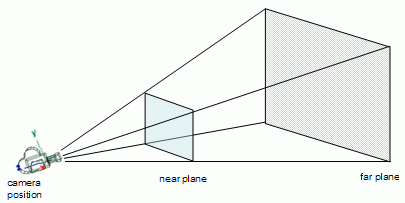
\includegraphics[width=0.8\linewidth]{visual_ambiguity.png}}
\end{center}
   \caption{Ambiguity of depth in single image.}
\label{fig:long}
\label{fig:onecol}
\end{figure}

For images of real scene, object prior is a clue to resolve the ambiguity of depth. While the object plane has infinite possible position, many of them corresponds to impractical real-world size of object. The basic equation in computer vision
\begin{equation}
\text{depth} \propto \text{focal\ length} * \frac{\text{real-world\ size}} {\text{size\ in\ photo}}
\end{equation}
implies that for fixed focal length and object size in photo(which is the case for single image depth estimation), depth of object is proportional to its real-world size. Through common knowledge and daily experience, we can extract some range so that most time size of the object is within such range. From the equation above, bounding the size of the object also gives a (typically tight) bound to its depth and thus provides strong information for depth. It implies that object size is of fundamental importance for depth estimation.

Some previous works \cite{} try to inject object prior by having human label depth directly. This kind of method typically labels several carefully-selected characteristic area. And depth of the rest region is worked out by propagation from labeled area. Such method fail to give satisfying results. Their failure lies mainly on the insensitivity of human to the absolute value of depth. Human are not good at labeling raw depth. To demonstrate our claim, we perform the simple experiment below: take 5 image with ground truth depth (collected by Kinect), randomly choose 10 pixel in every image and let 10 people label the raw depth of each pixel, compare the result with the ground truth. The final result shows roughly 21\% relative error which is far from accurate. Besides, long hesitation is observed before deciding the final depth, which indicates that it is also inefficient. So we make the conclusion that labeling raw depth is inadvisable.

Inspired by equation (1), we propose a method to label size instead. According to equation (1), for single image where focal length and object size in photo is fixed, depth is proportional to size and are thus equivalent. If we can get size by following the labeling-propagation process, relative depth is also known and absolute depth can be readily calculated given camera parameters. We find that labeling size can be much more accurate and efficient. Experimental result supports us: taking picture of common objects such as shelves, desks, chairs, measure their size, and let 10 people label the size, relative error decreases all the way down to 8\%, and most testers give their answer instantly. Thus conclusion can be made that labeling size is a better method for depth estimation, with higher efficiency and accuracy. 
%is prone to propagate errors, so depth labels in relatively high precision are required. However, manually labeling depth doesn't given satisfying accuracy(as we will show in the experiment section), which becomes a bottleneck for the method.

Despite the advantage of labeling depth, several challenge still remains to be tackled. The first problem is to decide the target to label. When labeling raw depth, pixel is a reasonable target to be labeled. But in our size-to-depth formulation, clue of depth comes from objects which is a semantic unit. It does not make sense to divide them into pixels. In addition, picking a representative pixel for an object is not trivial. But treating object as a whole necessitates the definition of object boundary. If we ask human to draw the boundary, it will be too time-consuming and the boundary will be noisy. We design a patch-to-size method to handle the problem with flexibility.

Propagation method is another concern. It has to figure out a way to preserve depth difference on object boundaries while remain the local connectivity of the depth map. The propagation method also need to tradeoff between fine-grained but computationally extensive high-resolution and coarse resolution with less computation expense. We apply conditional random field to do the propagation.

To sum up, we highlight the main contributions of this work as follows:
\begin{itemize}
\item We propose a new perspective for single monocular image depth estimation problem: from size to depth. Given manually labeled size for some objects in image, we are able to infer relative depth through simple geometric relationships. 
\item We design a special conditional random field (CRF) model to apply depth propagation and finally generate the whole depth map.
\item We demonstrate the superiorities of our method compared to the traditional depth-labeling method.
\end{itemize}

%In this paper, we propose a new method which estimates depth also by user interaction requiring size-related information from user instead of geometric or depth-related information. In our method, we firstly divide the image to be processed into small patches, and label approximate size for each patch. Then we... As human are able to describe the size of an object easier than to estimate the depth of an object in an image though daily experience, our method achieves good results and allows users to get rid of 

%-------------------------------------------------------------------------
\section{Related works}

Increasing number of methods are trying to estimate depth for single monocular image, which can be roughly classified into two families: learning-based method and interactive method.

Some traditional learning-based methods formulate depth estimation as a markov random field (MRF) learning problem. Saxena \etal \cite{NIPS2005_2921} use linear regression and MRF to predict depth from a set of image feature. Liu \etal \cite{Liu_2014_CVPR} propose a discrete-continuous conditional random field (CRF) model to take relations between adjacent superpixels into consideration. Realizing the strong correlation between depth estimation and semantic segmentation, Liu \etal \cite{Liu+al:CVPR10} make use of predicted semantic labels to guide 3D reconstruction by enforcing depth related to class and geometry prior.

Most of recent learning-based approaches rely on the application of deep learning, among which deep convolutional neural network (CNN) is used most commonly. Eigen \etal \cite{DBLP:journals/corr/EigenPF14} design a global coarse-scale deep CNN to regress a rough depth map directly from an input image. They then train a local fine-scale network to make local refinements. Liu \etal \cite{Liu_2015_CVPR} propose a deep convolutional neural field model for depth estimation by exploring CNN and  CRF. They jointly learn the unary and pairwise potentials of CRF in a unified deep CNN framework. Like in traditional learning-based method, Wang \etal \cite{Wang_2015_CVPR} use a deep CNN to jointly predict a global layout composed of pixel-wise depth values as well as semantic labels, and improved performance by allowing interactions between depth and semantic information. 

Compared to our method, learning-based methods require plenty of ground truth data and are not able to generalize to unseen images outside the dataset. Some of the methods \cite{Liu+al:CVPR10, Wang_2015_CVPR} need result of segmentation algorithm.

Human interactive methods exploit human ability to interpret 2D images, using human annotation. Some previous works make use of geometric elements (lines or plains) in images to predict depth. Criminisi \etal \cite{Criminisi2000} describe a way to compute 3D affine measurements given human inputs providing geometric information determined from the image. Later works \cite{Lee2009GeometricRF} by Lee \etal try to generate plausible interpretations of a scene from a collection of line segments automatically extracted from a single indoor image. These methods are limited for requiring a large amount of straight lines or plains in the image to provide enough evidences for 3D structure inference. Lopez \etal \cite{ceig.20141109} formulate the problem as an optimization process by assuming that image regions with low gradients will have similar depth values. In their method, depth values are propagated between pixels with small image gradients under a number of human-defined constraints. Our method, In contrast, requires only size information, which is more trivial for human to label than geometric or depth information. We will show this in the following sections.

\section{Our method}
In this section, we present details of our size-to-depth algorithm for depth estimation. We use bold upper case letter to denote matrices and bold lower case letter to denote vectors.

\subsection{Overview}
%Our goal is to estimate pixelwise depth for single image of general cases. The ability of inferring depth in human brain depends extensively on its knowledge of objects and their spatial relations. Inference of depth should be made on the basis of knowledge of 3d shape of real-world objects as well as understanding of 3d space. However, learning-based methods performing depth estimation is basically built on 2d images. Learning-based methods built on such data are forced to work out depth which requires 3d understanding given training information of lower dimension, introducing much ill-posedness to the problem.  Besides, RGBD datasets generated by devices like Kinect and Lidar is limited in both type of scene and number of images. Popular RGBD datasets such as NYU Depth or SUN RGBD typically contain images of indoor scenes less than or on the order of million. Such low dimension, biased and inadequate data is not sufficient for applying an NN-based method. Another point is, a model haven't been developed that has level of understanding of 3d space and spatial relation the task requires. We are still working on asking questions like counting number of objects which is a much much simpler problem than reasoning spatial relation in 3d space. Neither gain knowledge of 3d object shape nor inferring spatial relation is solved as a single problem, and learning-based methods are asking neural networks to do both for depth estimation. Thus, learning-based methods, at least in this time, is not sufficient to handle this task on its own. Senses of human are involved to be sensitive to comparing relative depth but not estimating raw value of depth. One can readily distinguish the nearer object between two, but struggles to name that distance to an object is 10m, 12m or 15m.
Our goal is to estimate pixelwise depth for single image of general cases. As directly labeling depth in numeric value is inefficient and inaccurate, we propose the quick and precise size-to-depth algorithm.

Following the labeling-propagation pipeline, the first step of our algorithm is labeling size which is an fast and efficient technique. According to equation (1), real-world size is proportional to depth in single image depth estimation setting. Thus size is equivalent to relative depth and we can calculate absolute depth given the camera parameters.
%To involve both local and global horizon, this is done several times for coarse-to-fine patch division of image.

After patch-to-size step, we obtain size for each patch (which is equivalent to depth). But the result is rather coarse with rigid boundary. Another depth refinement step is introduced to smooth depth gaps and interpolate between pixels under the constraint of depth annotation.

The depth refinement step is formulated as an energy function optimization problem in conditional random field (CRF). Mathematically, let $\mathbf{x}$ be the RGB image, $\mathbf{y}$ be the corresponding depth, we model the conditional probability distribution of data with
\begin{equation}
\text{Pr}(\mathbf{y}|\mathbf{x}) = \frac{1}{Z(\mathbf{x})}\text{exp}(-E(\mathbf{x}, \mathbf{y}))
\end{equation}
where $E(\mathbf{x}, \mathbf{y})$ is the energy function and $Z(\mathbf{x})$ is a normalization term given by
\begin{equation}
Z(\mathbf{x}) = \int_{\mathbf{y}}\text{exp}(-E(\mathbf{x}, \mathbf{y})) d\mathbf{y}.
\end{equation}

Maximum a posteriori (MAP) solution $\mathbf{y}^*$ gives the depth of maximum probability $\mathbf{y}$ for observed image $\mathbf{x}$ which is the best estimation of depth
\begin{equation}
\mathbf{y^*} = \text{argmax}_{\mathbf{y}} \log \text{Pr}(\mathbf{y}|\mathbf{x}).
\end{equation}
\par
In the following, we will give a detailed discussion about components of our algorithm.
\subsection{Annotation formulation}
Realizing the difficulty to model object knowledge and spatial relation, we introduce human annotation for additional information. Due to the urge to preserve the structure of sematic unit and the difficulty to pick representative pixel for certain object, we discard the scheme to label size at pixel level. But getting accurate object boundary requires extensive annotation labor or the inclusion of segmentation which will greatly degrade convenience and time complexity. We propose a patch-to-size method that tradeoff between the two cases and partially preserves structure of semantic unit while remains fast and convenient. In this formulation, image is divided into grids of equally sized patches. And human are asked to label real-world size of dominant component in each patch. The dominant component treatment keeps the structure of semantic units. It enables the semantically homogeneous pixels to be evenly constrained, which reduces computational cost. Meanwhile, dominant component does not deterministically specify certain object, avoiding the inconvenience and inefficiency of annotation introduced by the problem of defining object boundary. However, the obvious disadvantage of introducing dominant component is one have to wisely select the proper dominant component which requires certain level of experience.

We make the general assumption that depth of dominant component in the patch is representative of the entire patch (this does not mean we will assign same depth for every pixel in the patch, actually we are assigning same constraint, discussed later in Section 3.4). The assumption sounds inapplicable in some cases such as images depicting a person in the background of sky where depth in same patch may vary greatly. But it can be fixed by introducing CRF as shown in section 3.4.

\subsection{Conditional random field}
As is typically formulated, energy function of our CRF consists of unary and binary terms.
\begin{align}
E(\mathbf{x}, \mathbf{y}) &= \sum_{p \in P}E_{unary}(\mathbf{y}_{p}, \mathbf{x}) \notag \\ &\quad + \lambda \sum_{(b, c) \in A} \frac{1}{2} E_{binary}(\mathbf{y}_b, \mathbf{y}_c, \mathbf{x})
\end{align}
where $P$ is the set of pixels in the image, $A$ is set of 4-connected adjacent pair of pixels, $E_{unary}\text{ and }E_{binary}$ are relatively unary and binary terms, and $\lambda$ is a hyperparameter controlling the tradeoff of unary and binary term.

The unary term is given by
\begin{align}
E_{unary}(\mathbf{y}_{p}, \mathbf{x}) &= (\mathbf{y}_p - \mathbf{d}_p)^2
\end{align}
where $\mathbf{d}$ is the depth annotation. This term basically forces the depth of image to match with labeled depth of its belonging patches. It will constrain the global layout of depth map to be relatively reasonable. 


\par
The binary term is given by
\begin{equation}
E_{binary}(\mathbf{y}_b, \mathbf{y}_c, \mathbf{x}) = \text{sim}(b, c) (\mathbf{y}_b-\mathbf{y}_c)^2
\end{equation}

\begin{figure*}[!ht]
\begin{center}
\fbox{\rule{0pt}{0in} \rule{0\linewidth}{0pt}
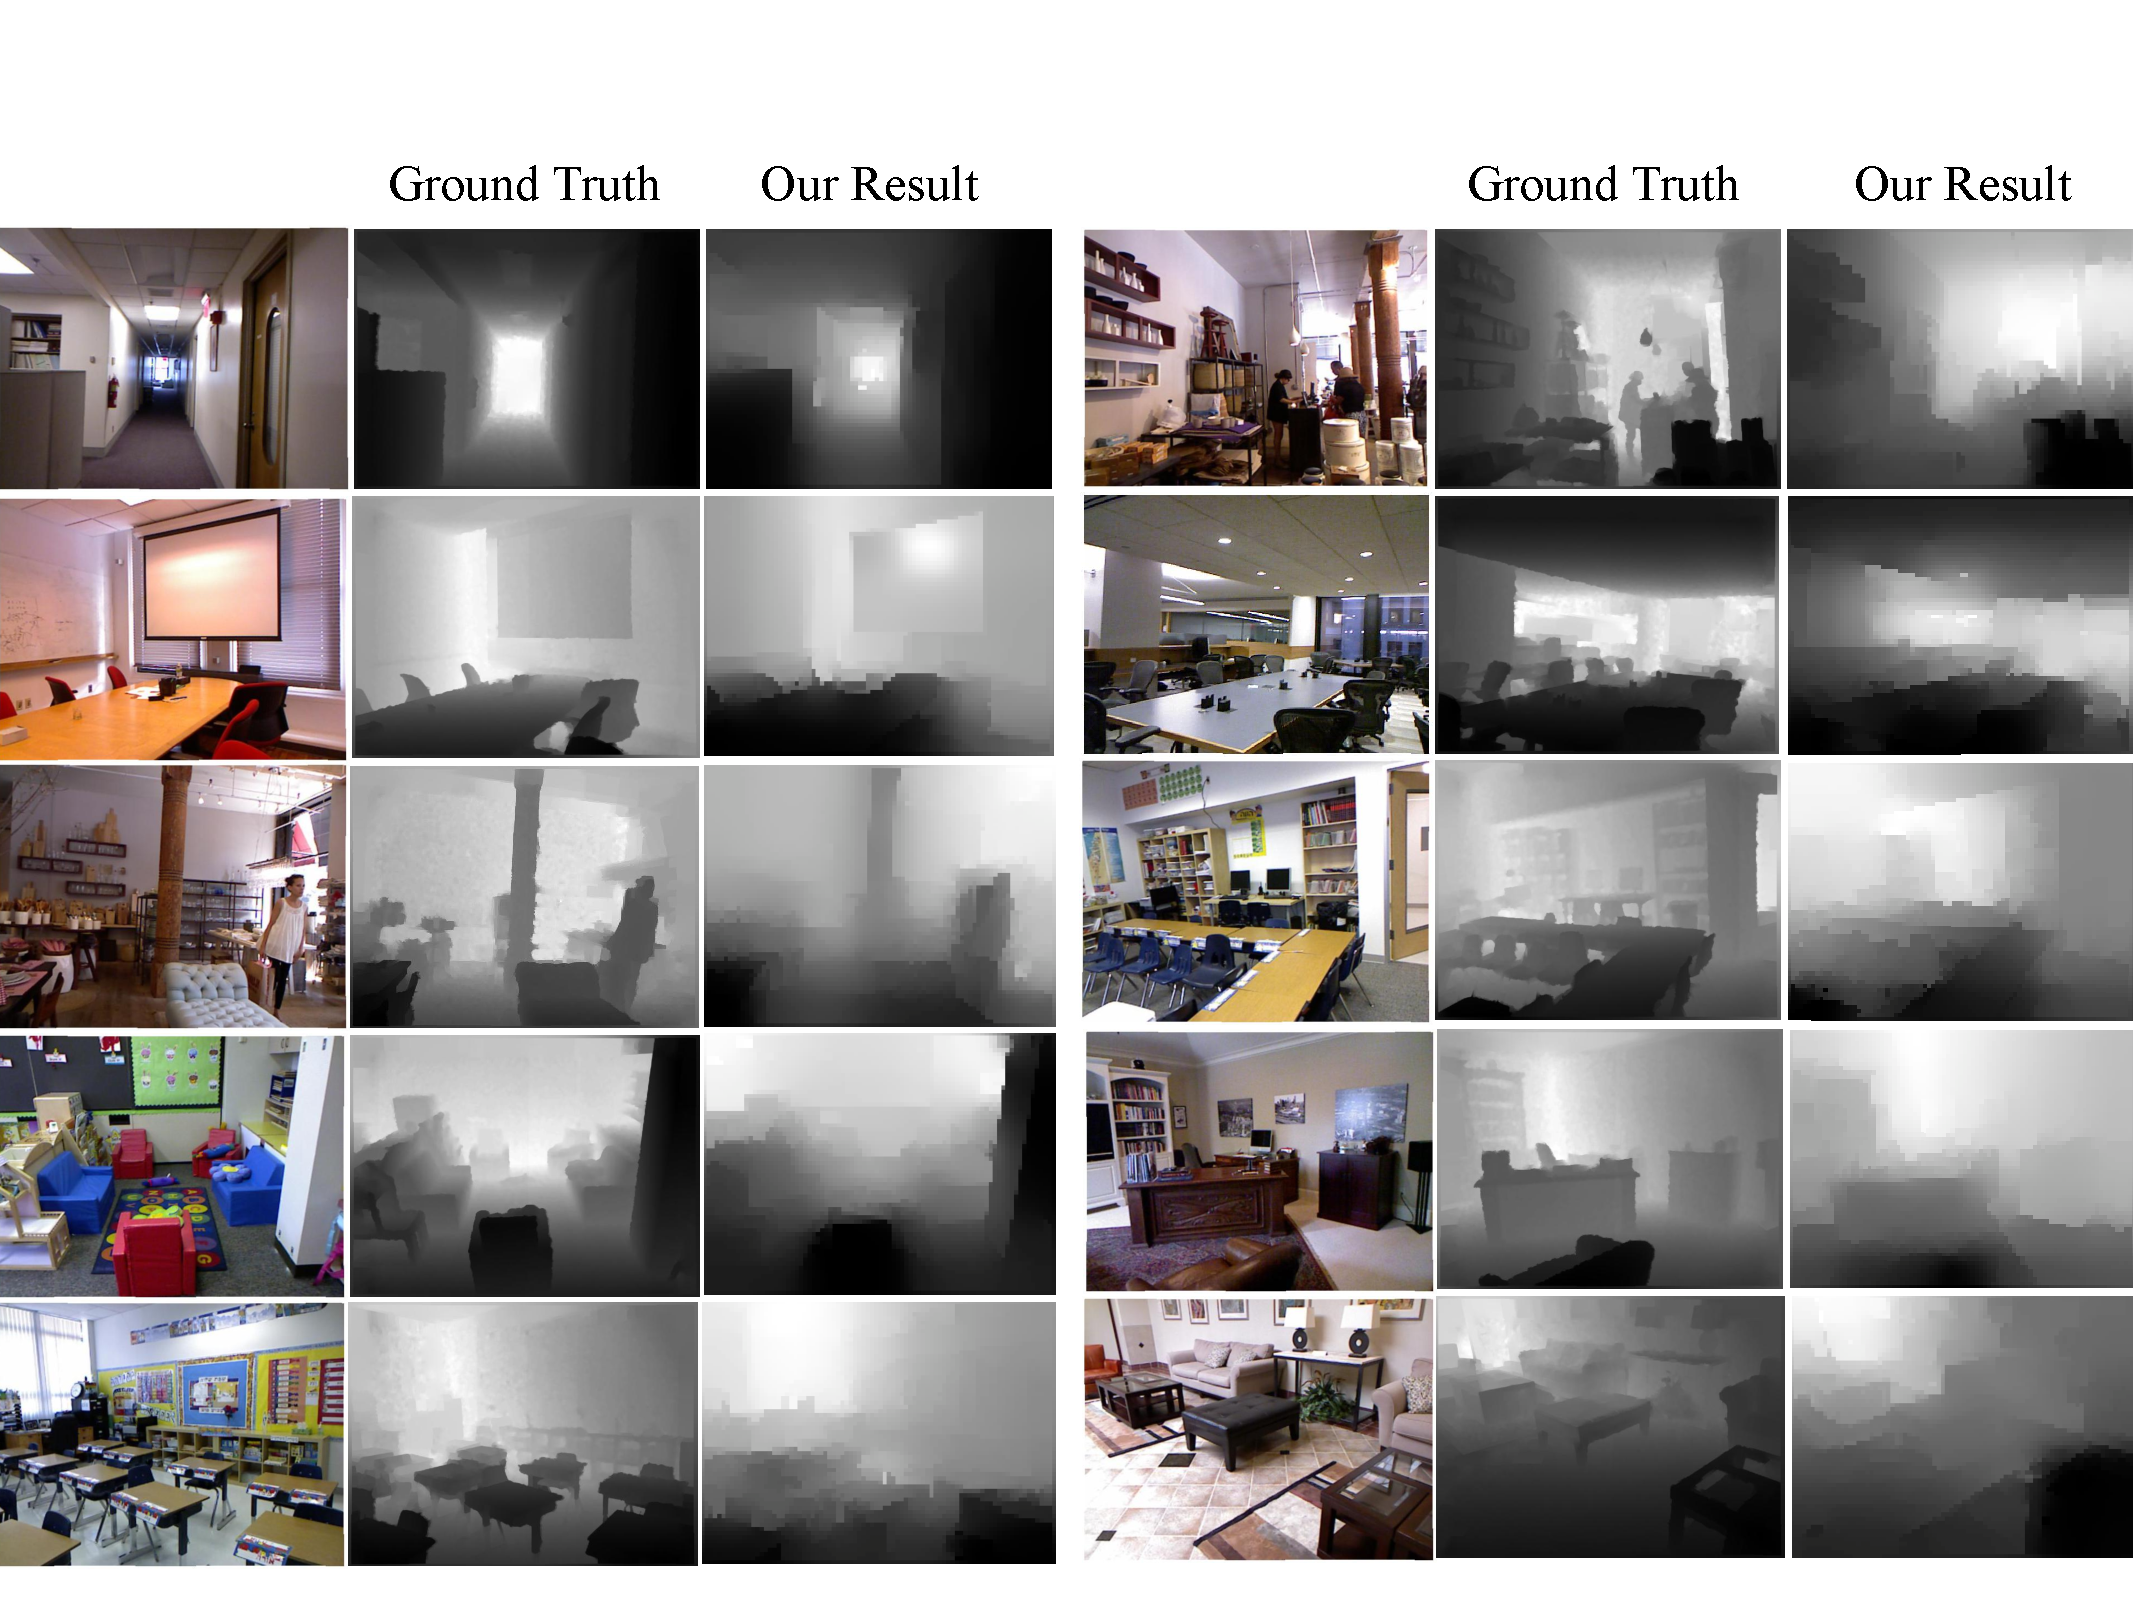
\includegraphics[width=17.5cm]{demos.pdf}}
\end{center}
   \caption{Results of our method on NYU Depth dataset. The left column contains original images. Ground truth depth maps are placed in the center column and our results are presented in the right column.}
\label{fig:short}
\end{figure*} 

where $\text{sim}(b, c)$ is a similarity function of pixel. This term penalizes gap of depth between neighboring pixels which encourages local continuity of the depth field.
Similarity function between pixels can be represented by image gradient
\begin{equation}
\text{sim}(b, c) = e^{-\beta (I_b-I_c)}
\end{equation}
where $I_b, I_c$ denotes image intensity at b, c, and hyper-parameter $\beta$ controls the strength of local continuity. Smaller $\beta$ corresponds to stronger continuity constraint.

\subsection{MAP in CRF}
In the case of manual annotation, depth $\mathbf{d}$ is predefined by user. And if we measure similarity by image gradient, energy function can be written as
\begin{align}
E(\mathbf{x}, \mathbf{y}) &= \sum_{p \in P} (\mathbf{y}_p-\mathbf{d}_p)^2 + \lambda \sum_{b, c \in A}\text{sim}(b, c)(\mathbf{y}_b-\mathbf{y}_c)^2 \notag \\
&= \mathbf{y}^T (\ I+\lambda(\ \text{diag}(\mathbf{s}) - W )\ )\mathbf{y}-2\mathbf{y}^T\mathbf{d}+\mathbf{d}^T\mathbf{d}  \notag
\\ &= \mathbf{y}^T W'\mathbf{y}-2\mathbf{y}^T\mathbf{d}+\mathbf{d}^T\mathbf{d} 
\end{align}
where $I$ is the identity matrix, $\mathbf{d}$ is the annotation vector, $W_{ij} = \text{sim}(i, j) $, $\mathbf{s}_i = \sum_j W_{ij}$ and

$W' = I+\lambda(\ \text{diag}(\mathbf{s}) - W ).$

\begin{equation}
\text{Pr}(\mathbf{y}|\mathbf{x}) = \frac{\mathbf{y}^T W'\mathbf{y}-2\mathbf{y}^T\mathbf{d}+\mathbf{d}^T\mathbf{d} }{Z(\mathbf{x})}
\end{equation}
The optimization is performed by taking gradient w.r.t $\mathbf{y}$.
\begin{align}
\frac{\partial{\text{Pr}(\mathbf{y}|\mathbf{x})}}{\partial\mathbf{y}} &= \frac{\mathbf{y} ^T(W'+W'^T)-2\mathbf{d}^T}{Z(\mathbf{x})} = 0 \notag \\
\mathbf{y} &= 2(W'+W'^T)^{-1}\mathbf{d}
\end{align}

\section{Experiment}
\subsection{Comparison with hand-crafted depth}
In this subsection, we design an experiment to compare depth calculated by our method with hand-crafted depth. 
\subsubsection{Evaluation procedure}
\text{\ \ \ \ }We use the following experiment procedure. For an arbitrary image, firstly we randomly pick $N$ (in our experiment, we take $N = 10$) points in image and ask human to directly label the depth of these points. Then we generate the depth map for the image using our method and write down the depth for the same $N$ points. We compare the depth of $N$ chosen points directly labeled by human and generated using our algorithm by following three metrics.

\subsubsection{Evaluation metrics}
\text{\ \ \ } Three metrics are used to evaluate the estimation result, \ie mean square error, cosine similarity with ground truth and pairwise rank accuracy. We use ground truth as our target. The formal definitions of these metrics are listed as follows:

\begin{itemize}
\item mean square error:
$\frac{1}{N} \sum_p{(d_p^{gt} - d_p)^2} $;
\item mean cosine similarity:
$ \frac{\bf{x}^{gt} \cdot \bf{x}}{|\bf{x}^{gt}| \cdot |\bf{x}|} $;
\item pairwise rank accuracy:\\
\begin{align*}
\frac{1}{N \cdot (N-1) / 2} &\sum_{p, p'}\mathbb{I} \{(d_p \leqslant d_{p'} \ and \ d_p^{gt} \leqslant d_{p'}^{gt}) \\
 &\ \ \ \ \ \  or\  (d_p \geqslant d_{p'} \ and \ d_p^{gt} \geqslant d_{p'}^{gt}) \};
\end{align*} 
\end{itemize}
where $N$ is the total number of pixels in all the evaluated image, $d_p^{gt}$ and $d_p$ are the ground truth and predicted depth respectively at pixel indexed by $p$, and $\mathbf{x}^{gt}$ and $\mathbf{x}$ are $T$-dimensional vectors whose components are $d_p^{gt}$ and $d_p$, respectively.

\subsection{Performance on NYU Depth dataset}

\begin{table}
\begin{center}
\begin{tabular}{|l|c|c|}
\hline
Metric             & Size to Depth & Hand-crafted Depth\\ 
\hline
Mean Square Error  & 0.016     & 0.048 \\
Cosines Similarity     & 0.976    & 0.935 \\
Pairwise Accuracy  & 0.858     & 0.818 \\
\hline
\end{tabular}
\end{center}
\caption{Result on three metrics. Depth generated by our method outperforms hand-crafted depth.}
\end{table}

We test images from NYU Depth dataset \cite{silberman11indoor, Silberman:ECCV12} and use our algorithm to generate depth map for them. Processing a standard image with size $480 \times 640$ takes tens of seconds. Some of the results are shown in Figure 2. 

\section{Conclusion}
We have presented a size to depth method for single monocular image depth estimation. The proposed method exploit the strength of human to estimate object size.  We explain the superiors of human labeling size compared to labeling depth. We show that the size labeled by human can be transferred to depth information through geometric relationships. A specific CRF model then propagate depth to generate the whole depth map. Experiments show that our method outperforms traditional depth-labeling method and generates quite satisfactory depth maps.


{\small
\bibliographystyle{ieee}
\bibliography{egbib}
}


\end{document}
